\makeatletter
\def\input@path{{../}}
\makeatother

\documentclass[/main.tex]{subfiles}

\begin{document}
\graphicspath{{./pics/}{ch1/pics/}}

\onlyinsubfile{\textpages}
\chapter{The Theory of Neutrino Mass and Double-Beta Decay}

\section{A Brief History of Neutrinos}
\subsection{Discovery of Neutrinos}
Nuclear radioactivity was discovered and characterized at the turn of the twentieth century by a group of physicists including Henri Becquerel, Marie Curie and Ernest Rutherford.
The three main types of decay studied were:
\begin{itemize}
\item $\alpha$-decay, in which a \iso{4}{He} nucleus is ejected from a nucleus
\item $\beta^-$-decay, in which an electron is emitted from a nucleus and a neutron inside the nucleus becomes a proton
\item $\gamma$-decay, in which a nucleus in an excited state decays to the ground state and emits a high energy photon in the process
\end{itemize}
In the cases of $\alpha$- and $\gamma$-decays, the particles are emitted monoenergetically, with kinetic energies that can be predicted using energy conservation by the change in mass between the parent and daughter nuclei, according to
\begin{equation}
  E=mc^2
\end{equation}
However, extensive experimental efforts by Lise Meitner, Otto Hahn, Jean Danysz, James Chadwick, Charles Drummond Ellis, and others established that $\beta$-decay has a diffuse energy spectrum that could not be explained through energy conservation; furthermore, angular momentum conservation appeared to be violated in these decays.
In 1930, Wolfgang Pauli proposed that this broad spectrum could instead be explained by a small, non-interacting, spin-1/2 particle that escapes the nucleus along with the electron, and carries away undetected kinetic energy, thus conserving energy and angular momentum.

\begin{figure}[t]
  \centering
  \subfloat[Beta Decay]{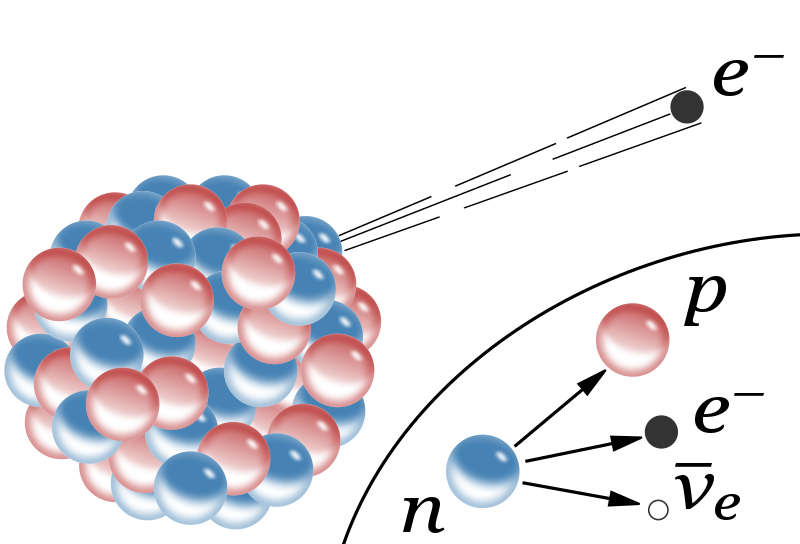
\includegraphics[width=0.35\textwidth]{beta}}
  \subfloat[Fermi Decay Diagram]{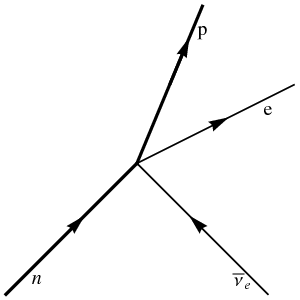
\includegraphics[width=0.25\textwidth]{fermidiagram}}
  \subfloat[Energy Spectrum]{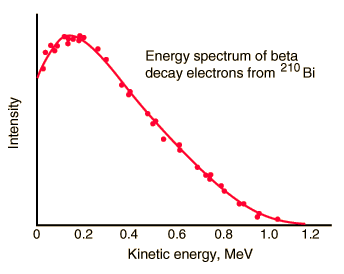
\includegraphics[width=0.35\textwidth]{betaspectrum}}
  \caption[Beta decay and energy spectrum]{\label{fig:beta}
    A beta decay emits an electron while transmuting a neutron into a proton. The energy spectrum of the electron is broad instead of peak-like (measured by G.J. Neary (1940), taken from \url{http://hyperphysics.phy-astr.gsu.edu/hbase/Nuclear/beta2.html}).
  }
\end{figure}
By 1934, Enrico Fermi proposed a theory of $\beta$-decay that included Pauli's neutral particle, a spin 1/2 electrically neutral particle he named the neutrino ($\nu$)\cite{Fermi1934}.
The Lagrangian for the Fermi interaction is
\begin{equation}
  \mathcal{L}_F=\frac{G_F}{\sqrt{2}}\big(\bar \psi_p \gamma^\mu \psi_n\big)\big(\bar \psi_e \gamma_\mu \psi_\nu\big)
\end{equation}
This theory was capable of describing the broad energy spectrum of $\beta$-decay, and also capable of describing nuclear $\beta^+$-decay, in which a positron is emitted and a nuclear proton becomes a neutron.
Furthermore, this theory predicted the process of inverse $\beta$-decay, in which a neutrino is absorbed by a nucleus, and either an electron is produced with a proton becoming a neutron, or a positron is produced with a neutron becoming a proton.
Fermi's theory, however, predicted a cross-section for inverse $\beta$-decay on the order of $\sigma\approx10^{-44}~\mathrm{cm}^2$, meaning that a single neutrino would have a mean free path on the order of light-years through lead.
Due to the extremely low cross-section, the force mediating the interactions described by Fermi's theory became known as the weak force.
Pauli, Fermi and the Nature review board were all understandably pessimistic about the possibility of actually detecting this newly predicted process, resulting in Nature's refusal to publish Fermi's theory\cite{Pais1988}.

This pessimism, however, was unwarrented.
Twenty years later, Reines and Cowan detected the inverse $\beta$-decay in a water target using liquid scintillator detectors\cite{Cowan1957}.
This experiment was enabled by the high flux of neutrinos produced by the Savannah River nuclear reactor.
Specifically, Reines and Cowan detected the production of positrons by inverse $\beta^-$-decay of protons in the water.
Other attempts to detect electrons produced by inverse $\beta^+$-decay from neutrinos produced in a reactor failed to measure anything \cite{Davis2002}.
This is explained by the existence of distinct neutrinos ($\nu$) and anti-neutrinos ($\bar{\nu}$).
Weak interactions are expected to conserve the quantity of Lepton Number ($L$), where electrons and neutrinos have $L=+1$ and positrons and anti-neutrinos have $L=-1$.
This means that $\beta^+$-~and inverse $\beta^+$-decays will involve neutrinos, and $\beta^-$~and inverse $\beta^-$-decays will involve anti-neutrinos.
Since the Savannah River nuclear reactor produced almost entirely anti-neutrinos via $\beta^-$-decays, the only interaction detected involved the production of positrons via inverse $\beta^-$-decay.
To date, no interaction has been observed that violates Lepton-number conservation.

\subsection{Parity Violation in the Weak Force}
The discrete parity symmetry (P) is conserved for the electromagnetic and strong forces.
In 1956, Lee and Yang suggested that the discrete parity symmetry (P) could be violated by the weak force, as no experimental evidence existed to confirm or reject this\cite{LeeYang1956}.
Within a year, Wu and collaborators experimentally demonstrated P violation by placing \Co{60} under a strong magnetic field at low temperature and by measuring the correlation between the directions of the deexcitation $\gamma$s and of the electron emitted.
If P is conserved, no correlation is expected in these directions; however, Wu found an anti-correlation, implying P-violation\cite{Wu1957}.
Shortly after, Garwin, Lederman and Weinrich confirmed this in the polarization of muons produced by decays of pions in flight\cite{Garwin1957}.

In 1958, Goldhaber and collaborators observed that the weak force is maximally parity violating, and weak interactions involve only left-handed neutrinos\cite{Goldhaber1958}.
This result, combined with contemporary results that were consistent witha massless neutrino\cite{PDG2018}, meant that there was no experimental evidence for the existence of right-handed neutrinos.
For this reason, neutrinos were presumed to be strictly left-handed, represented by massless Weyl spinors.
In addition, the weak Lagrangian was modified to be
\begin{equation}
  \mathcal{L}_W=-\frac{G_F}{\sqrt{2}}\big(\bar \psi_p \gamma^\mu \frac{1-\gamma^5}{2} \psi_n\big)\big(\bar \psi_e \gamma_\mu \frac{1-\gamma^5}{2} \psi_\nu\big)
\end{equation}
Due to P violation, the Fermi vertex has a vector-axial~vector (V-A) tensor structure.

\subsection{Flavors of Neutrinos}
In addition to the electron, additional charged elementary particles with identical properties (e.g. spin, charge) to the electron, except for mass, exist\cite{PDG2018}.
These are the muon ($m_\mu=113$~MeV) and tau lepton ($m_\tau=1.8$~GeV), which are unstable due to their high masses.
The existence of three different particles with similar properties except for mass is mirrored in quarks (the constituents of protons and neutrons and other ``baryons''), and the different types are called ``flavors'', with the different mass groupings called ``generations''.
Both heavy leptons decay via the weak force, producing neutrinos in the process.
The neutrinos produced in these decays can subsequently undergo processes analogous to inverse beta decay, producing either muons or tau leptons instead of electrons, and maintaining conservation of lepton number.
Furthermore, over short distances, it was observed that these neutrinos produced the same particle as those which created them.
This means that there are three distinct types of neutrinos corresponding to the three types of lepton; these are called the electron neutrino ($\nu_e$), muon neutrino ($\nu_\mu$), and tau neutrino ($\nu_\tau$).
The weak decay of a muon into an electron looks like:
\begin{equation}
  \mu \rightarrow e + \nu_\mu + \bar \nu_e
\end{equation}
The fact that the flavor of leptons appeared to be conserved was in contrast with quarks, where a weak decay could transmute quarks between different generations.

\subsection{Electroweak Unification}
During the 1930's-50's, a large number of new particles were discovered, with properties and interactions that could be described using the algebra of Lie groups.
Between 1961 and 1967, Glashow, Weinberg and Salam proposed a theory of electro-weak unification, a theory which simultaneously described the electromagnetic and weak interactions with a U(1) gauge symmetry representing weak hypercharge and a SU(2) gauge symmetry representing isospin (i.e. a SU(2)$\times$U(1) gauge symmetry)\cite{Glashow1962, Weinberg1967, Salam1968}.
This theory predicted the existence of the $\mathrm{W}^{+/-}$ boson, a heavy, electrically charged, spin~1 particle which forms interaction vertices with electrons and neutrinos or with up and down quarks, which are the components of protons and neutrons.
As shown in Figure~\ref{fig:betadecayW}, this theory is capable of reproducing the vertex in Fermi's theory of weak interaction, with the W boson acting as a mediator for $\beta$-decay.
The W~boson interacts only with left-handed particles, and the effective charged-current interaction term lagrangian at energies below the electroweak symmetry breaking scale is:
\begin{equation}
  \mathcal{L}_C=-\frac{g}{\sqrt{2}}\big(\bar u_i \gamma^\mu \frac{1-\gamma^5}{2} M^{CKM}_{ij}d_j + \bar \nu_i \gamma_\mu \frac{1-\gamma^5}{2} e_i\big)W^+_\mu + \mathrm{h.c.}  
\end{equation}
where $M^{CKM}_{ij}$ is the Cabibbo-Kobayashi-Maskawa (CKM) matrix that describes the probability of a weak transition between different generations of quark, and $i$ and $j$ index over the generations.
\begin{figure}[t]
  \centering
  \subfloat{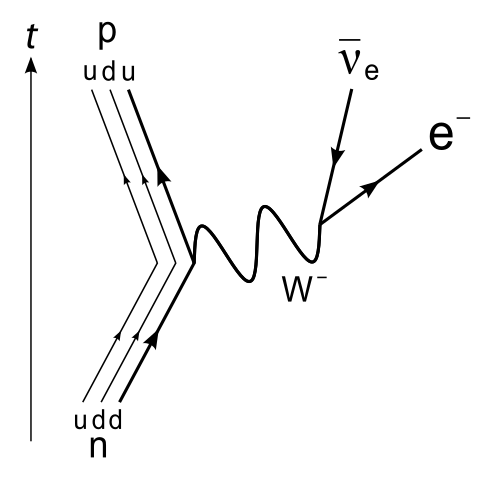
\includegraphics[width=0.4\textwidth]{betadiagram}}
  \subfloat{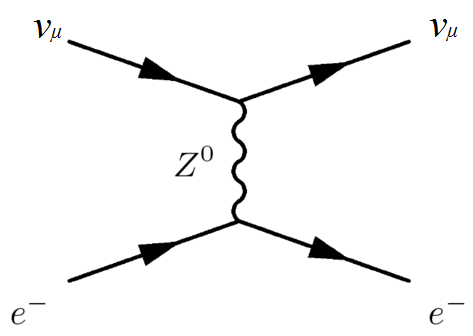
\includegraphics[width=0.4\textwidth]{neutralcurrentscatter}}
  \caption[$\beta$-decay diagram with W]{\label{fig:betadecayW}
    Diagrams of $\beta$-decay mediated by the W-boson and of a neutral current scatter of a neutrino off an electron, mediated by the Z-boson.
  }
\end{figure}

This theory also made a number of new predictions, which have since been confirmed.
The Z~boson, a heavy, neutral, spin~1 boson was predicted, which would enable elastic scattering of neutrinos off other weakly interacting particles.
Neutrino elastic scattering of a muon neutrino off of an electron was observed by the Gargamelle detector in 1973\cite{Gargamelle1973}, and both the W~and Z~bosons were observed at the Super Proton Synchotron in 1983\cite{Arnison1983, Bagnaia1983}.
This theory also incorporated the Higgs boson, a spin~0 boson that imparts mass to the fermions in the standard model, as will be discussed in Section~\ref{sec:diracmass}.
The Higgs boson was discovered at the ATLAS and CMS detectors using the Large Hadron Collider in 2012\cite{ATLAS2012, CMS2012}.

\subsection{The Standard Model of Particle Physics} \label{sec:SM}
\begin{figure}[t]
  \centering
  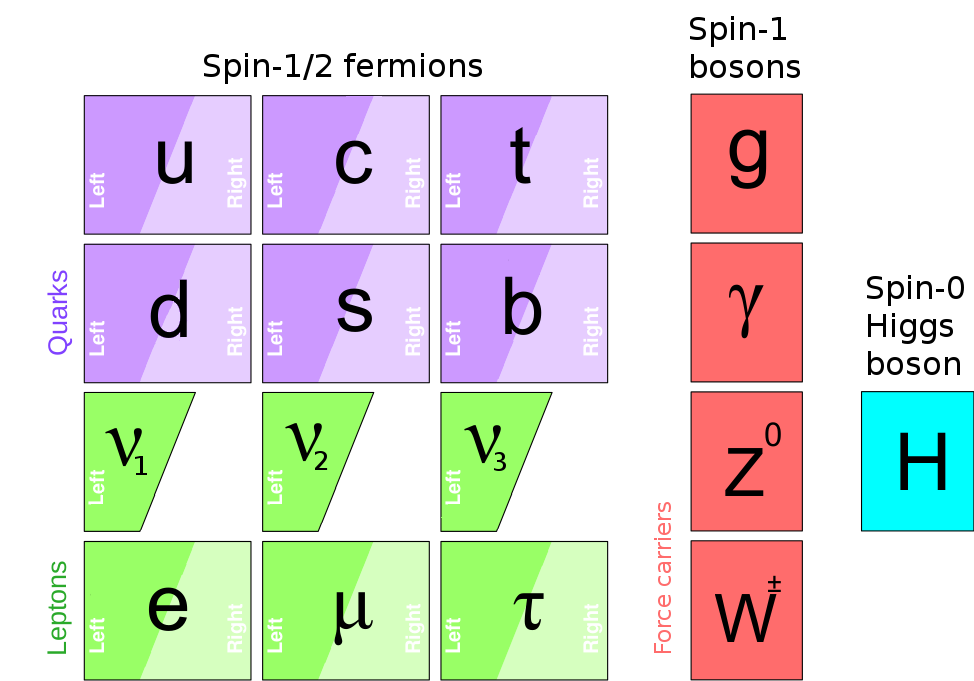
\includegraphics[width=0.8\textwidth]{SM}
  \caption[Standard Model Particles]{\label{fig:SM}
    Diagram of all standard model particles.
  }
\end{figure}
Over the course of the 1960's through~80's, this electroweak unification scheme was expanded into a theory called the Standard Model, based on a U(1)$\times$SU(2)$\times$SU(3)~gauge symmetry, with the non-Abelian SU(3) component describing the strong force \cite{PDG2018}.
All of the fundamental particles included in this theory are summarized in Figure~\ref{fig:SM}.
This theory included five integer-spin bosons:
\begin{itemize}
\item The photon ($\gamma$) mediates electromagnetism, and only interacts with electrically charged particles
\item The W and Z bosons mediate the weak force, and only interact with left-handed fermions
\item 8 types of gluons, with different ``color'' charges, mediate the strong force, and only interact with quarks
\item The Higgs boson imparts mass to all the other particles, except for the massless photons and neutrinos
\end{itemize}
The spin-1/2 fermions include the rest of the particles, and are divided into four groups, with 3 generations each:
\begin{itemize}
\item Up-type quarks (up (u), charm (c) and top (t)) have electrical charge +2/3 and interact via the EM, weak and strong forces
\item Down-type quarks (down (d), strange (s) and bottom (b)) quarks have electrical charge -1/3 and interact via the EM, weak and strong forces
\item Charged leptons (e, $\mu$ and $\tau$) have charge -1, and interact via the EM and weak forces
\item Neutrinos ($\nu_e$, $\nu_\mu$ and $\nu_\tau$) have no charge and interact only via the weak force. In addition, they are massless, and have only left-handed components
\end{itemize}
\begin{table}[h]
  \caption[Weak properties of Fermions]{\label{tab:doubsing}
    Table of weak properties of the Standard Model fermions. Note the lack of right-handed neutrino singlets.
  }
  \centering
  \begin{tabular}{|c|c|c c|c c c|}
  \hline
  Fermion & Electric& & Weak & \multicolumn{3}{c|}{Generation}\\
  type & Charge & & isospin & 1 & 2 & 3 \\
  \hline
  \multirow{2}{*}{Quarks} & \multirow{2}{*}{$+\frac{2}{3}$,$-\frac{1}{3}$} & doublet & $\frac{1}{2}$ & $\begin{pmatrix}u\\d\end{pmatrix}_L$ & $\begin{pmatrix}c\\s\end{pmatrix}_L$ & $\begin{pmatrix}t\\b\end{pmatrix}_L$ \\
          & & singlet & 0 & $u_R$, $d_R$ & $s_R$, $c_R$ & $t_R$, $b_R$ \\
  \hline
  \multirow{2}{*}{Quarks} & \multirow{2}{*}{$-1$, $0$} & doublet & $\frac{1}{2}$ & $\begin{pmatrix}e\\ \nu_e\end{pmatrix}_L$ & $\begin{pmatrix}\mu\\ \nu_\mu\end{pmatrix}_L$ & $\begin{pmatrix}\tau\\ \nu_\tau\end{pmatrix}_L$ \\
          & & singlet & 0 & $e_R$ & $\mu_R$ & $\tau_R$ \\
  \hline
\end{tabular}
\end{table}
Because the weak force only interacts with left-handed particles, each grouping is divided into a left-handed doublet and right-handed singlets, as shown in Table~\ref{tab:doubsing}.
The Standard Model has been extensively tested for interactions between the particles included therein, and with few exceptions, has been verified.
It is, however, incomplete, failing to describe gravity, dark matter, the accelerating expansion of the universe, the matter asymmetry of the universe, and other natural phenomena; this not-yet-described physics is referred to as Beyond the Standard Model (BSM).

Lepton number and Baryon number ($B$, the total number of Baryons\textemdash composites of three quarks, minus anti-Baryons) are both conserved in low energy interactions in the Standard Model, including the weak force.
At energies above the electroweak unification scale (${\sim}1$~TeV), however, the nonperturbative ``sphaleron'' process is capable of violating both $B$ and $L$ conservation.
Figure~\ref{fig:sphaleron} shows how a sphaleron can occur if a system is heated above the sphaleron energy and then cools into a different vaccuum state, with different Lepton- and Baryon-numbers.
\begin{figure}[t]
  \centering
  \subfloat[Vacuum Potential]{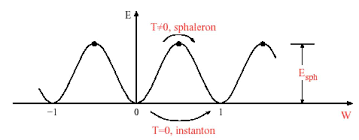
\includegraphics[width=0.5\textwidth]{sphaleronpotential}}
  \subfloat[Sphaleron]{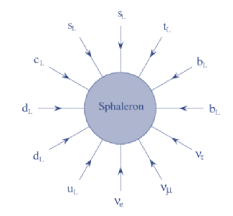
\includegraphics[width=0.4\textwidth]{sphaleron}}
  \caption[Standard Model Sphaleron]{\label{fig:sphaleron}
    Left: The periodic vacuum potential of the Standard Model as a function of essentially $B+L$. If the temperature of a system is brought above $E_{sp}$, the system can re-cool into a state with different $B+L$.\\
    Right: A sphaleron diagram generating $\Delta B = -\Delta L = 3$
  }
\end{figure}
The simplest process would increment or decrement both $L$ and $B$ by~3; any such process would conserve the value of $B-L$, as this is an exact, accidental symmetry of the Standard Model.
Because of the extreme energies required for this process to occur with any significant probability, it has never been observed; however, this process would occur during the early universe, with consequences that will be briefly discussed in Section~\ref{sec:implications}.

\section{Discovery of Neutrino Mass}
\subsection{The Solar Neutrino Problem}
\begin{figure}[t]
  \centering
  \subfloat[Illustration of the pp-fusion process]{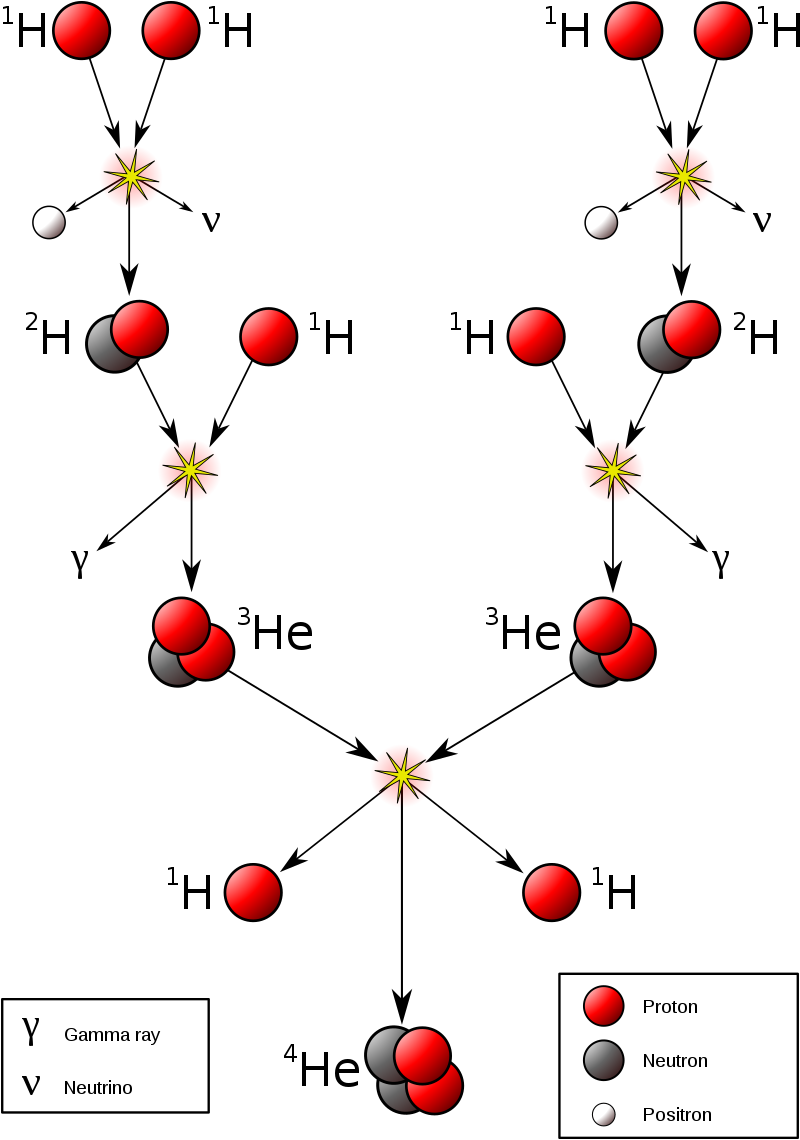
\includegraphics[height=7.5cm]{pp_process}}
  \subfloat[Solar neutrino energy spectrum]{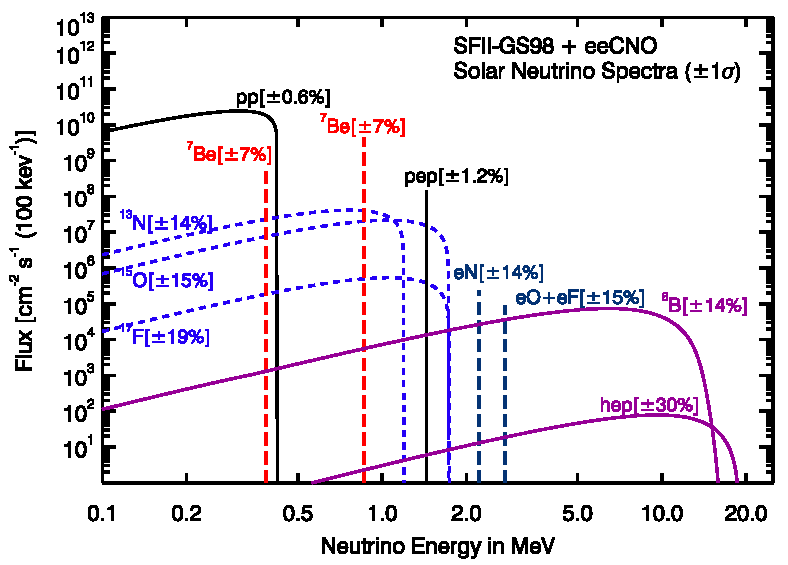
\includegraphics[height=7.5cm]{solarnuspectrum}}
  \caption[Neutrinos produced by Solar fusion]{\label{fig:ppproc}
    The energy spectrum of neutrinos produced by the Sun (right) can be predicted by understanding the fusion processes that occur (such as the pp-process, left). Taken from \cite{PDG2018}.
  }
\end{figure}
The first hint of BSM physics in neutrinos came from the Solar Neutrino problem.
During the various processes involved in nuclear fusion in the Sun, numerous neutrinos are produced; for example, the pp-process, which is the dominant process for producing \iso{4}{He} from \iso{1}{H}, produces two neutrinos per \iso{4}{He} nucleus (see Figure~\ref{fig:ppproc}).
Solar models can predict the number and energy spectrum of neutrinos emitted by various production channels in the Sun\cite{Bahcall2005}.
In 1962, Davis began to directly measure the flux of solar neutrinos in the Homestake mine in South Dakota by counting inverse $\beta$-decays of \iso{37}{Cl} into \iso{37}{Ar}.
Over multiple decades of measurement, Davis consistently measured one third as many neutrinos as expected\cite{Cleveland1998}.
Additional experiments observed similar deficits, including SAGE and GALLEX, which measured inverse $\beta$-decays with a lower energy threshold than the Homestake experiment using \iso{71}{Ga}\cite{SageGallex1999}.

\subsection{Neutrino Mass Mixing}
One (among many) explanation for this deficit is neutrino mixing, which was predicted by Pontecorvo in 1957\cite{Pontecorvo1957}, and further developed by Maki, Nakagawa and Sakata in 1962\cite{Maki1962}.
Under this model, neutrinos are described by mass eigenstates, $\nu_1$, $\nu_2$ and $\nu_3$, which describe how the neutrinos move freely through space.
The neutrinos of the Standard Model, now called flavor eigenstates, are coherent quantum admixtures of the mass eigenstates, and describe how neutrinos interact weakly with other particles.
In 1969, Pontecorvo proposed neutrino oscillation as an explanation for the observed deficit of Solar neutrinos\cite{Pontecorvo1969}.

Mathematically, mixing is described by the Pontecorvo-Maki-Nakagawa-Sakata (PMNS) matrix ($U^{\mathrm{PMNS}}$), which is unitary.
In the example of a $\beta$-decay, the electron anti-neutrino emitted is the following superposition:
\begin{equation}
  \ket{\bar\nu_e}=U^*_{1e}\ket{\bar\nu_1}+U^*_{2e}\ket{\bar\nu_2}+U^*_{13}\ket{\bar\nu_3}
\end{equation}
The PMNS matrix can be written as
\begin{equation} \label{eq:PMNS}
  \begin{pmatrix}
    U_{e1} & U_{e2} & U_{e3} \\
    U_{\mu1} & U_{\mu2} & U_{\mu3} \\
    U_{\tau1} & U_{\tau2} & U_{\tau3}
  \end{pmatrix} = \begin{pmatrix}
    1 & 0 & 0 \\
    0 & c_{23} & s_{23} \\
    0 & -s_{23} & c_{23}
  \end{pmatrix} \cdot \begin{pmatrix}
    c_{13} & 0 & s_{13}e^{-i\delta} \\
    0 & 1 & 0 \\
    -s_{13}e^{i\delta} & 0 & c_{13}
  \end{pmatrix} \cdot \begin{pmatrix}
    c_{12} & s_{12} & 0 \\
    -s_{12} & c_{12} & 0 \\
    0 & 0 & 1
  \end{pmatrix}
\end{equation}
where $s/c_{ij}$ are the sines and cosines of the mixing angles $\theta_{ij}$ and $\delta$ is a CP-violating term known as the CP-phase.
During neutrino oscillation, the probability of measuring a neutrino in a weak eigenstate changes according to (in the approximation of only two neutrinos):
\begin{equation}
  P_{\alpha\rightarrow\beta}=\sin^2\left(2\theta_{ij}\right)\sin^2\left(\frac{(\Delta m^2)_{ij}c^3}{4\hbar E}L\right)
\end{equation}
where $(\Delta m^2)_{ij}$ is the difference in the squares of the masses of the neutrino mass eigenstates $i$ and $j$, $L$ is the distance from the neutrino source, and $E$ is the energy of the neutrino.
The neutrinos oscillate as a function of $L/E$, with a frequency proportional to $\Delta m^2$.
This mixing in the Lepton sector is similar to mixing of quarks via the CKM~matrix, which enables flavor changing weak decays in mesons and baryons.

\subsection{Discovery of Neutrino Oscillation}
\begin{figure}[t]
  \centering
  \subfloat[SuperK $\nu$ Oscillation Signal]{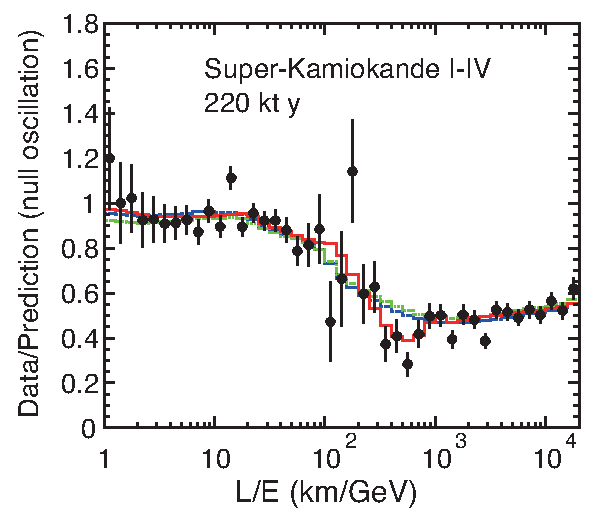
\includegraphics[height=4cm]{superkoscillation}}
  \subfloat[SNO $\nu$ Mass Mixing Signal]{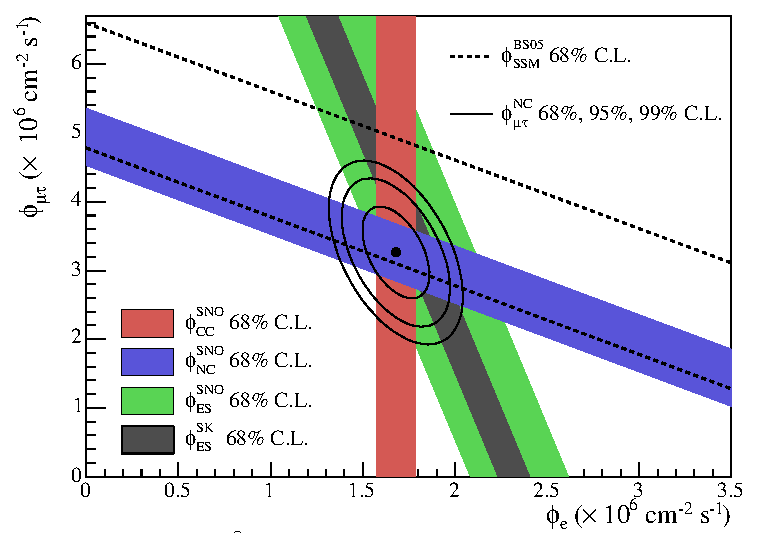
\includegraphics[height=4cm]{snonumixing}}
  \subfloat[KamLAND $\nu$ Oscillation Signal]{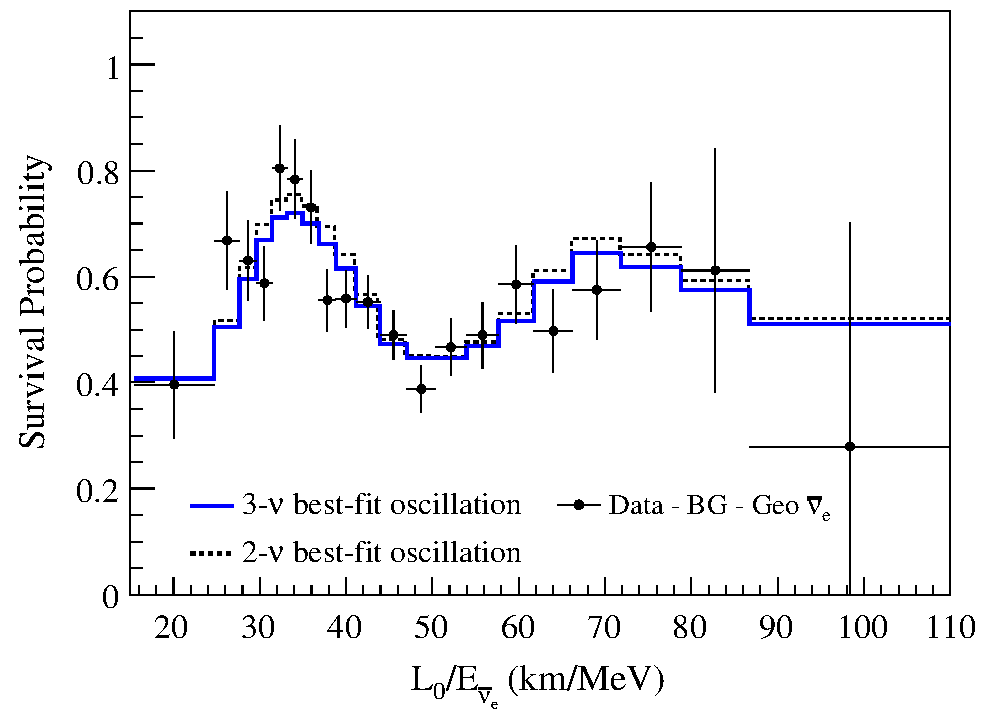
\includegraphics[height=4cm]{kamlandoscillation}}
  \caption[Confirmation of Neutrino Oscillation]{\label{fig:nuoscillation}
    The signals of neutrino mixing from disappearence of atmospheric $\nu_\mu$s in SuperKamiokande, difference in total solar-$\nu$ flux and solar-$\nu_e$ flux from SNO, and disappearence of reactor $\nu_e$s in KamLAND. Taken from \cite{PDG2018}}
\end{figure}
  In 1998, SuperKamiokande, observed a deficit of atmospheric muon neutrinos dependant on the zenith angle, consistent with neutrino oscillation\cite{superk1998}.
In 2000, the SNO experiment observed neutrino flavor mixing in solar neutrinos.
Since solar $\nu_e$s are produced amid an extremely high electron density, as they escape the Sun, they will adiabatically transform into the $\nu_2$ eigenstate due to the MSW effect.
By observing solar neutrinos via different interaction mechanisms, SNO had sensitivity to both the total number of neutrinos, regardless of flavor, via neutral current interactions, and to the number of electron neutrinos via charged current interactions.
SNO observed the expected total number of neutrinos according to the Standard Solar Model\cite{Bahcall2005}, while observing a deficit in electron neutrinos, definitively solving the Solar Neutrino Problem\cite{SNO2002}.
Finally, in 2003 KamLAND observed a deficit of electron neutrinos from nuclear reactors consistent with oscillation\cite{kamland2003}.
Figure~\ref{fig:nuoscillation} shows the results of all three experiments.
Between these three measurements, a deficit has been observed in Solar, atmospheric, and reactor neutrinos, and this deficit has been explained in a simple and consistent way using the PMNS mass mixing model.

\begin{figure}[t]
  \centering
  \subfloat[Neutrino Oscillation Parameters]{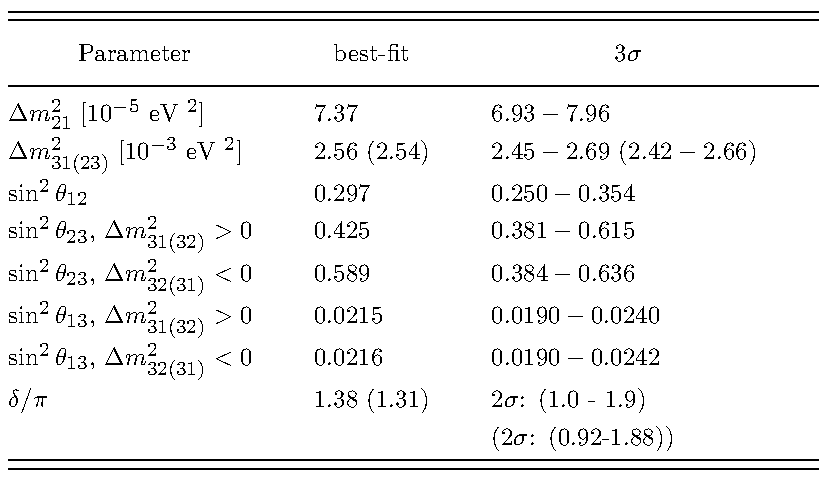
\includegraphics[width=0.5\textwidth]{oscillationparameters}}
  \subfloat[Mass Ordering]{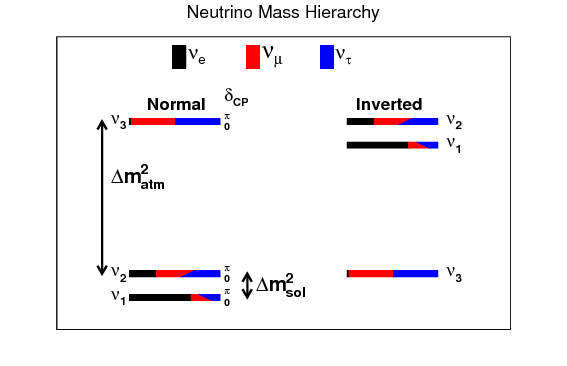
\includegraphics[width=0.45\textwidth]{numassordering}}
  \caption[Neutrino Oscillation Parameters and Mass Ordering]{\label{fig:massordering}
    Left: Table of measured neutrino parameters from oscillation experiments, taken from \cite{PDG2018}.\\
    Right: Solutions of neutrino mass ordering that are consistant with oscillation results.
  }
\end{figure}
An extensive experimental program of oscillation experiments has since measured all of the mixing angles in the PMNS matrix, and the $\Delta m^2$ parameters, as shown in Figure~\ref{fig:massordering}.
Even so, many questions remain.
First, the absolute masses of the neutrinos are unknown.
Second, the sign of $\Delta m^2_{32}$ is unknown, resulting in two possible orderings for the neutrino masses.
These are referred to as the ``Normal'' ordering, in which $m_3>m_2>m_1$, and the ``Inverted'' ordering, in which $m_2>m_1>m_3$, as shown in Figure~\ref{fig:massordering}.
Third, the CP-phase of the PMNS-matrix, $\delta$, has not been measured.
Fourth, the possibility for additional, heavier neutrinos that do not interact via the weak force, but do mix with the other neutrinos, exists.
Finally, and of greatest interest to this document, the mechanism for granting mass to neutrinos is currently unknown.
As will be discussed in Section~\ref{sec:numasstheory}, the Standard Model does not allow for neutrino mass, and multiple possible mechanisms exist for granting it.


\section{Theory of Neutrino Mass} \label{sec:numasstheory}
The Standard Model of Particle Physics includes only left-handed neutrinos.
The Lagrangian represents neutrinos as left-handed Weyl spinors, representing a left-handed (LH) particle and a right-handed (RH) anti-particle.
A CPT transformation, flips between a LH particle and RH anti-particle; due to CPT invariance, these must have identical properties except for helicity and charge, meaning this is the simplest possible representation of a spin-$\frac{1}{2}$ particle.
However, we now understand that neutrinos are massive, which cannot be explained without extending the Standard Model.
This section will discuss possible mechanisms for generating neutrino mass and why extension of the Standard Model is required for each.
For a more detailed and complete discussion, see C.~Giunti and C.W.~Kim, Chapter 6~\cite{Giunti}.

\subsection{A Brief Discussion of Helicity and Chirality} \label{sec:helicitychirality}
So far, this document has been loose in its description of handedness, which can refer to either helicity or chirality.
The helicity operator ($h$) is defined as
\begin{equation}
  h=\mathbf{\frac{s\cdot p}{|p|}}=\frac{p_1[\gamma^2,\gamma^3]+p_2[\gamma^3\,\gamma^1]+p_3[\gamma^1\,\gamma^2]}{2|\mathbf{p}|}
\end{equation}
where $\mathbf{s}$ is spin, $\mathbf{p}$ is particle momentum, and $\gamma^i$ are Dirac matrices.
Helicity can be equivalently described as the particle spin projected onto its momentum.
The chirality operator ($\gamma^5$) is defined as 
\begin{equation}
  \gamma^5=i\gamma^0\gamma^1\gamma^2\gamma^3
\end{equation}
Furthermore, for massless particles (and in the ultra-relativistic limit for massive particles), helicity and chirality eigenstates are identical, with equal eigenvalues for particles and opposite eigenvalues for anti-particles.

For massive particles, helicity is not Lorentz invariant, while chirality is.
This can be intuitively seen by imagining a massive, classical fermion moving through free space from frames of reference moving slower and faster than it.
When switching between these frames, the spin direction will appear the same, while the direction of momentum will flip, meaning that the helicity will flip as well.
For this reason, the helicity operator cannot appear as a part of the Standard Model Lagrangian while chirality can.
This means that Fermion spinors are eigenstates of chirality, and the weak force interacts directly with left-chiral states rather than left-helicity states.
On the other hand, for massive particles, helicity is a constant of motion since momentum and angular momentum are both conserved, while chirality is not.

\subsection{Dirac Mass} \label{sec:diracmass}
All other Standard Model fermions gain mass via the Dirac mechanism, and are called Dirac fermions\cite{Dirac1928}.
A Dirac fermion is represented by a Dirac spinor, which consists of a left-handed Weyl spinor paired with a right-handed one.
Dirac spinors represent the states used to solve the Dirac equation which describes the wavefunction for a free, relativistic, spin-1/2 particle:
\begin{equation}
  i\gamma^\mu \partial_\mu \psi - m\psi = 0
\end{equation}
In the standard model lagrangian, a Dirac mass term appears as:
\begin{equation}
  \mathcal{L}_{Dirac}=-m\bar\nu\nu=m(\bar\psi_L\psi_R+\bar\psi_R\psi_L)
\end{equation}
This represents a coupling between a left- and right-handed fermion.

In the Standard Model, a bare mass term is forbidden because the fermions are not invariant under SU(2) gauge transformations, due to the doublet structure of the left-handed fermions.
A mass term is introduced by the Higgs field, which is a spin-0 doublet $\Phi=\begin{pmatrix} \phi^+ \\ \phi_0\end{pmatrix}$.
The $\phi^+$ field is charged and the $\phi_0$ field is neutral, and therefore able to take on a vacuum expectation value:
\begin{equation}
  \Phi(x)=\frac{1}{\sqrt{2}}\begin{pmatrix}  0\\ v+H(x)\end{pmatrix}
\end{equation}
where $v$ is the vacuum expectation and $H(x)$ is the field that produces the Higgs Boson.
Through the Higgs, then, we can introduce mass to a Standard Model fermion in the doublet $\begin{pmatrix}f' \\ f\end{pmatrix}_L$ and singlet $f_R$:
\begin{equation}
  \mathcal{L}_{Y}=-g\begin{pmatrix}\bar f' & \bar f\end{pmatrix}_L \cdot\frac{1}{\sqrt{2}}\begin{pmatrix}0 \\ v+H(x)\end{pmatrix} f_R = -\frac{gv}{\sqrt{2}}\bar f_Lf_R
\end{equation}
where $g$ is the coupling of the fermion to the Higgs field.
To introduce Dirac mass to the neutrino, we would have to add a right-handed neutrino singlet to the standard model with a non-zero Higgs coupling.

\subsection{Majorana Mass}
A second mechanism for granting mass to neutral fermions exists, called the Majorana mechanism\cite{Majorana1937}.
In this case, fermions are the solutions to the Majorana equation:
\begin{equation}
  i\gamma^\mu\partial_\mu\psi - m\psi^C = 0
\end{equation}
where $\psi^C$ is the charge-conjugated field:
\begin{equation}
  \psi^C=\mathcal{C}\bar\psi^T
\end{equation}
The Majorana equation is solved by a two-component Majorana spinor consisting of a single left-chiral spinor or right-chiral spinor:
\begin{equation}
  \psi=\psi_{L/R}+\psi_{L/R}^C
\end{equation}
where $\psi_{L/R}$ are left/right-handed Weyl spinors.
For a Majorana fermion, the mass term in the Lagrangian is:
\begin{equation}
  \mathcal{L}_{Majorana}=-m\bar{\psi^C}\psi=-m(\bar{\psi^C}_L\psi_L + \bar\psi_L\psi^C_L)
\end{equation}
This represents a coupling between a left-handed particle and a right-handed anti-particle.
Because of this mass coupling, the electric charge of the fermion is no longer a constant of motion; this means that only a neutral fermion can possibly have Majorana mass, making the neutrino the only Standard Model particle that could possibly be a Majorana fermion.
Similarly, lepton number is no longer a constant of motion, which would enable lepton-number violating processes.
For this reason, we often say that a Majorana particle is its own anti-particle.

The Standard Model, however, forbids a bare Majorana mass term, once again due to the SU(2) doublet structure of the left-handed leptons.
Such a term would appear as:
\begin{equation}
  \mathcal{L}_{Majorana}=-m\left(\begin{pmatrix}\bar e & \bar\nu\end{pmatrix}_L\begin{pmatrix}e^C \\ \nu^C\end{pmatrix}_L + h.c.\right)
\end{equation}
which would violate electric charge conservation due to the electron term.
If the Standard Model is an effective field theory for a more complete model with BSM physics at higher energy scales, a dimension five term could be introduced to the Lagrangian that generates Majorana mass:
\begin{equation} \label{eq:dimfive}
  \mathcal{L}_5= -\frac{g}{\Lambda}(L^T_L\tau_2\Phi)C^\dagger(\Phi^T\tau_2L_L) + h.c. = -\frac{gv^2}{2\Lambda}\bar{\nu^C}_L\nu_L + h.c.
\end{equation}
where $L_L$ is a lepton doublet and $\Phi$ is the Higgs doublet, and $\Lambda$ is the energy scale of the BSM physics involved.
Several possible BSM diagrams that generate this dimension five term are shown in Figure~\ref{fig:dimfive}.

If neutrinos are Majorana, the PMNS matrix is allowed to have additional CP phases as follows:
\begin{equation}
  U^{\mathrm{PMNS}}_{MJ}=U^{\mathrm{PMNS}}_D\cdot\begin{pmatrix}
    e^{i\alpha_1/2} & 0 & 0 \\
    0 & e^{i\alpha_2/2} & 0 \\
    0 & 0 & 1
  \end{pmatrix}
\end{equation}
where $U^{\mathrm{PMNS}}_D$ is the PMNS matrix as described in equation~\ref{eq:PMNS}, $U^{\mathrm{PMNS}}_{MJ}$ is the PMNS matrix modified for Majorana neutrinos, and $\alpha_1$ and $\alpha_2$ are the Majorana CP phases.

\subsection{Why are Majorana Neutrinos Compelling?} \label{sec:implications}
If neutrinos are Majorana particles, it would potentially help to answer additional questions about the universe.
One such question is why neutrinos are so much lighter than all the other Standard Model fermions.
Current upper limits on neutrino mass are $\sqrt{\sum_{i=0}^{3}|U_{ei}|^2m_i^2}<2$~eV from direct mass measurements and $\sum_{i=0}^3m_i<(0.3-1.3)$~eV from cosmological measurements, depending on model assumptions\cite{PDG2018}.
\begin{figure}[t]
  \centering
  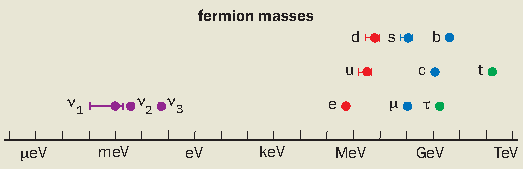
\includegraphics[width=0.9\textwidth]{numasssmall}
  \caption[Mass of Standard Model Fermions]{\label{fig:SMfermionmasses}
    Comparison of the masses of fermions in the standard model. Current limits place six orders of magnitude between the heaviest neutrino and the electron. Taken from H. Murayama, Physics World (2002).
  }
\end{figure}
As shown in Figure~\ref{fig:SMfermionmasses}, these limits place nearly six orders of magnitude difference in mass between the heaviest neutrino and the lightest charged fermion, which is larger than the log-scale difference between the lightest and heaviest charged fermion!
While this doesn't strictly require explanation, it is an unusual feature of the Standard Model if neutrinos gain their mass via the same mechanism as the other fermions.
Because the dimension five operator generates neutrino mass of $\frac{gv^2}{\Lambda}$, and where $gv^2$ is the square of a mass term generated by coupling a fermion to the Higgs field, and $\Lambda$ is expected to be at an energy scale beyond the electroweak unifcation scale, the mass generated would likely be very small.
Since this dimension five operator produces very light neutrino masses from the addition of heavy particles, the mechanisms for producing mass are often referred to as see-saw mechanisms.

Another mystery is why the universe consists of a significant amount of Baryonic matter (i.e. ``normal'' matter).
Under the Standard Model and the big bang theories, one would expect in the early universe to create large amounts of matter and anti-matter, which would annihilate leaving almost no matter in the universe.
Sakharov proposed three conditions necessary to generate the matter that we see\cite{Sakharov1967}:
\begin{itemize}
\item Baryon number violation
\item C and CP violation
\item B-, C-, and CP-violating process must happen out of thermal equilibrium
\end{itemize}
Since the Sphaleron process described in Section~\ref{sec:SM} is capable of converting lepton number into baryon number, Lepton number conservation would similarly suffice to generate a baryon number asymmetry.
A process that generates Majorana neutrino mass would also violate lepton number conservation and generate additional CP violation, potentially solving this mystery.

\subsection{Mechanisms for Generating Majorana Mass}
\begin{figure}[t]
  \centering
  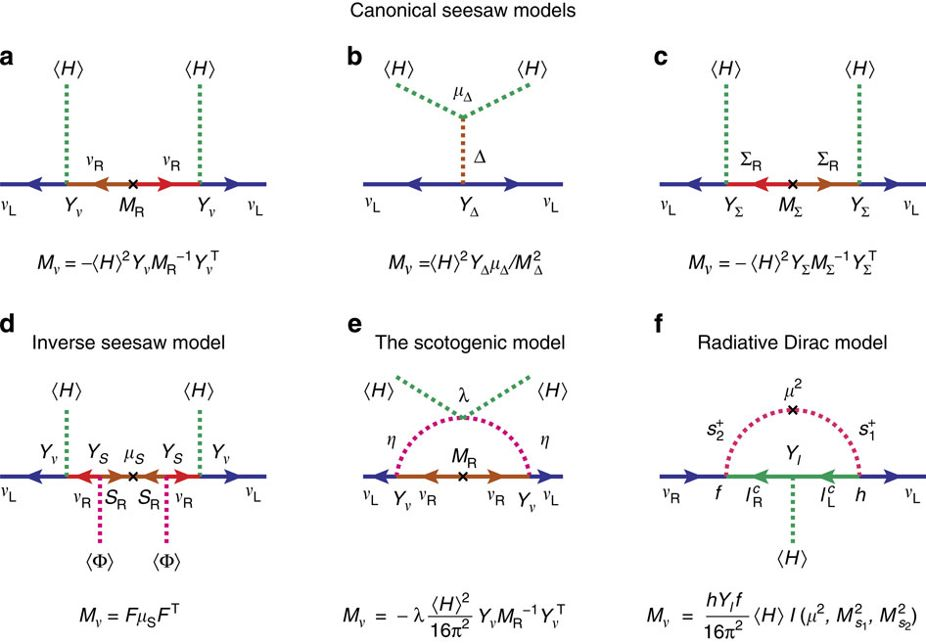
\includegraphics[width=0.9\textwidth]{dim5operator}
  \caption[Examples of Majorana Mass Generating Mechanisms]{\label{fig:dimfive}
    Examples of BSM mass generating mechanisms. Mechanisms a-e all reduce to the dimension five operator in equation~\ref{eq:dimfive} in a low energy effective theory. See referece~\cite{Ohlsson2014}.
  }
\end{figure}
This section will briefly discuss an incomplete list of BSM theories that could generate the dimension five operator that creates Majorana neutrino mass.
For more detailed descriptions of these theories, see \cite{Rodejohann2015, Perez2015}.
\begin{itemize}
\item \textbf{Minimal Extention of the Standard Model ($\nu$MSM)}: The simplest extention of the Standard Model that would produce Majorana neutrino mass is to simply add a right-handed neutrino singlet, $N$.
  This neutrino would be sterile, meaning it would not interact with any of the force carrying Bosons of the Standard Model.
  A right-handed neutrino would enable the addition of a Dirac mass term $m_D$, and since it would be an SU(2) singlet, also a Majorana mass term $M_R$.
  In this case, the mass term of the Lagrangian would appear as:
  \begin{equation}
    \mathcal{L_{\nu\mathrm{SM}}} = \begin{pmatrix} \bar{\nu^C}_L & \bar{N^C}_R \end{pmatrix} \begin{pmatrix} 0 & m_D \\ m_D & M_R \end{pmatrix} \begin{pmatrix} \nu_L \\ N_R \end{pmatrix}
  \end{equation}
  The mass matrix can be diagonalized, resulting in a left-chiral eigenstate with mass $\frac{m_D^2}{M_R}$ and a heavy, right-chiral eigenstate with mass $\approx M_R$.
  This process of generating a light, left-handed Majorana mass from a heavy right-handed neutrino is called the Type~I see-saw mechanism (letter a in Figure~\ref{fig:dimfive}).
  If the Dirac masses are at a similar energy scale to the other Standard Model fermions, and the right-handed mass is between the electro-weak and GUT energy scales, it is possible to generate neutrinos with masses similar to what we see.
\item \textbf{Left-Right Symmetric Model (LRSM)}: This model adds an additional SU(2) gauge symmetry that results in a second weak force that acts only on right-chiral particles.
  The right-handed symmetry breaking scale is at higher energies than the left-handed one, with the result that the right-chiral weak force interacts even less strongly than the left-chiral weak force.
  Under this model, the right-handed Fermions gain a doublet structure, requiring the addition of a right-handed neutrino.
  Additional Higgs fields are also required, resulting in a pair of Higgs triplets.
  This term would interact with both the right- and left-handed lepton doublets, generating Dirac and Majorana mass terms.
  Because the right-handed electroweak symmetry breaking scale is much higher than the left-handed one, this model would produce a light left-handed Majorana neutrino and a heavy right-handed Majorana neutrino.
  This is an example of a type~II mixed with a type~I see-saw mechanism (b~and~a in Figure~\ref{fig:dimfive}).
\item \textbf{SU(5) or SO(10) Grand Unified Theory (GUT)} SU(5) and SO(10) are the two smallest simple Lie groups that contain SU(3)$\times$SU(2)$\times$U(1) as a subgroup, making them popular groups for Grand Unified Theories.
  These GUTs violate lepton and baryon number, introducing particles called Leptoquarks.
  They also predict proton decay with a half-life that could be feasibly detected\cite{SuperK:pdecay}.
  SU(5) GUTs are disfavored by such measurements, while SO(10) GUTs will be investigated in future experiments.
  GUTs often add an additional fermion triplet that would induce a Majorana mass in the neutrino via a type~III and type~I see-saw mechanism (c~and~a in Figure~\ref{fig:dimfive}).
\item \textbf{R-Parity Violating Super-Symmetry (RPV SUSY)}: SUSY models add bosonic super-symmetric partners for each Standard Model fermion and vice-versa.
  R-parity is a discrete symmetry within SUSY; an R-parity transformation switches between a particle and its super-symmetric partner.
  Versions of SUSY that violate R-Parity symmetry enable Baryon and Lepton number violation, and in particular can add a Majorana neutrino mass.
\end{itemize}
The $\nu$MSM, as the minimal extension (only one particle added) needed to generate neutrino mass, is the typical model used when discussing Majorana neutrinos.
The other models mentioned, while more complex, may also solve other problems in physics for which the Standard Model is insufficient.
Due to their complexity, these other models will likely be observable through channels other than neutrino mass, such as scattering events at high energy colliders.

\section{Double-Beta Decay}
The only feasible way to determine whether or not the neutrino is a Majorana particle is to search for neutrinoless double-beta decay.
Two-neutrino double-beta (\tnbb) decay is an allowed second-order process in the standard model.
Neutrinoless double-beta (\znbb) decay is a hypothetical process that depends on the Majorana nature of the neutrino.
This section will describe both two-neutrino- and neutrinoless- double-beta decay, and discuss the theory for calculating the half-lives of each.
\begin{figure}[t]
  \centering
  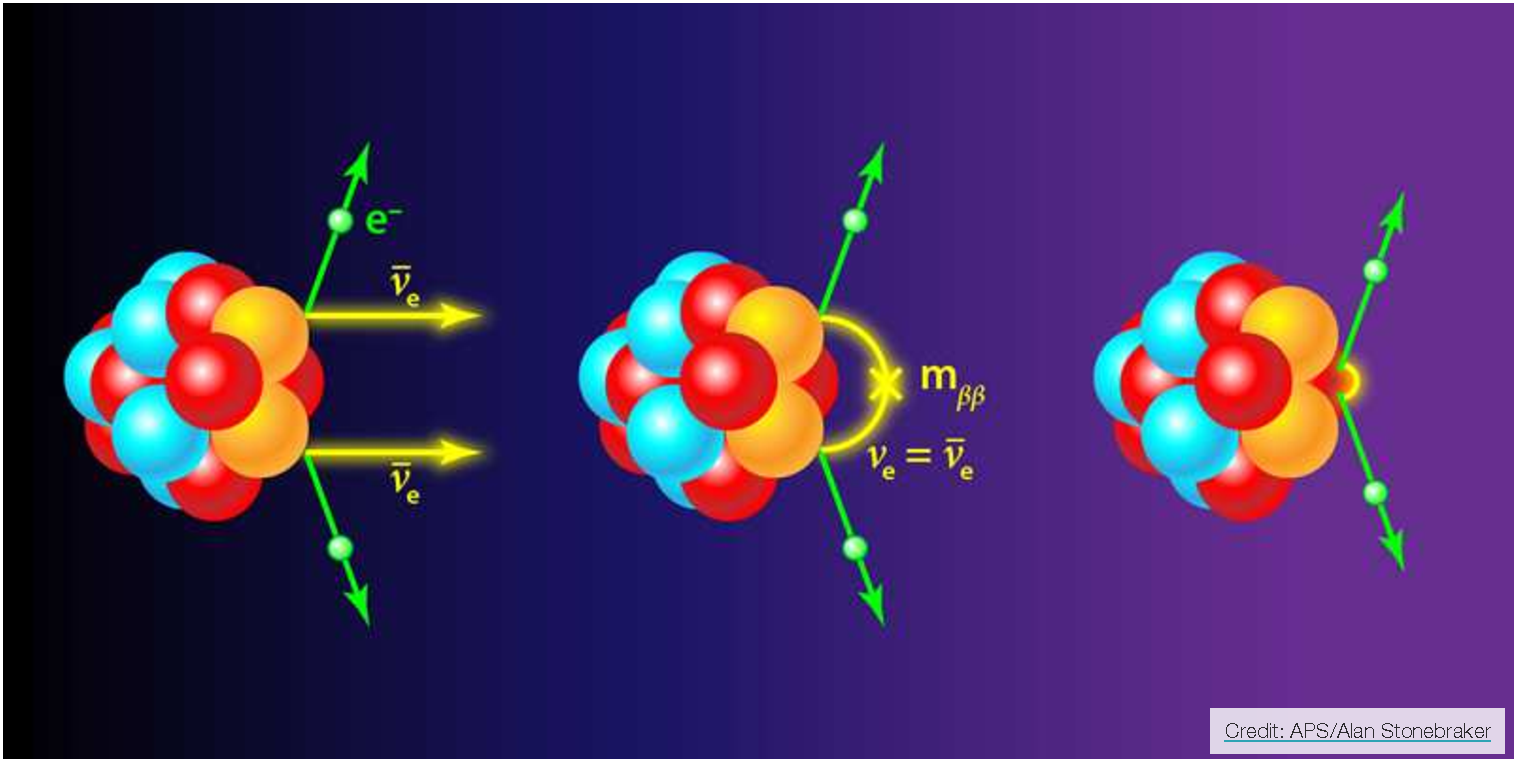
\includegraphics[width=0.8\textwidth]{bbdecay}
  \caption[Double-Beta Decay]{\label{fig:bbdecay}
    A drawing of three possible modes of double-beta decay. Left: \tnbb; Center: \znbb\ via light neutrino exchange; Right: \znbb\ via a short range mechanism
  }
\end{figure}

\subsection{Two-neutrino Double-Beta Decay}
During \tnbb\ decay, two neutrons inside a single nucleus become two protons, two electrons and two electron anti-neutrinos, equivalent to two simultaneous single $\beta$-decays.
\bb -decay is only observable in cases where single $\beta$-decay is energetically forbidden (with the exception of \iso{48}{Ca}, whose single $beta$-decay has a half-life $>10^{19}$~y).
As shown in Figure~\ref{fig:bballowed}, this situation occurs in nuclei with even numbers of nucleons: due to pairing interactions among protons and neutrons, odd-odd nuclei have higher masses than even-even nuclei, which can lead to single $\beta$-decay being forbidden while \bb -decay is allowed.
\begin{figure}[t]
  \centering
  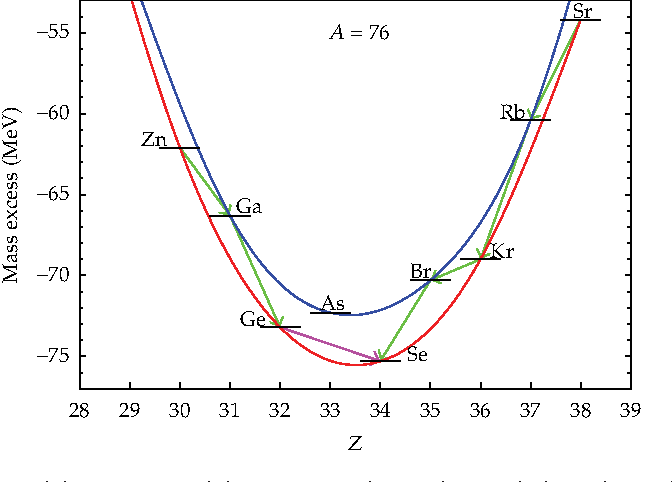
\includegraphics[width=0.8\textwidth]{bballowed}
  \caption[Allowed $\beta\beta$ Isobar]{\label{fig:bballowed}
    Energy levels of isotopes along the $Z=76$ isobar. The splitting of the even-even (red) and odd-odd (blue) nuclei is due to pairing interactions. In this case, \Ge{76} $\beta\beta$-decay into \Se{76} is observable because the single $\beta$-decay into \iso{76}{As} is energetically forbidden. Taken from J. Menendez's dissertation.
  }
\end{figure}
Because of the two neutrinos, which will carry kinetic energy out of any detectors, \tnbb\ has a broad energy spectrum as shown in Figure~\ref{fig:bbspectrum}, similar to single $\beta$-decay.
\begin{figure}[t]
  \centering
  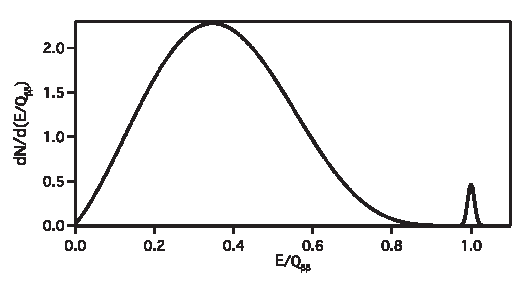
\includegraphics[width=0.8\textwidth]{bbSpectrum}
  \caption[Energy Spectrum of \tnbb\ and \znbb]{\label{fig:bbspectrum}
    Spectrum of electron energies in double-beta decay. The broad spectrum is due to \tnbb, while the peak at the Q-value is due to \znbb\ and, in the spectrum shown, has an amplitude of 1\% that of the \tnbb\ spectrum. Taken from \cite{Avignone2008}.
  }
\end{figure}
\bb -decay was predicted in 1935 by Goeppert-Mayer\cite{GoeppertMayer1935}, and was first measured using geochemical techniques in \iso{130}{Te} in 1950\cite{Inghram1950}, and directly in \iso{82}{Se} in 1987\cite{Elliott1987}.
\tnbb\ is possible in 35 naturally occuring isotopes, and has been detected in 11, with half-lives ranging from $10^{18}$~y to $10^{24}$~y\cite{Saakyan2013}.

\subsection{Calculating Half-life for \tnbb}
The half-life for \tnbb\ can be expressed, per Fermi's Golden Rule, as:
\begin{equation} \label{eq:2nvvHL}
  \frac{1}{T^{2\nu}_{1/2}}=G_{2\nu}(Q,Z)(g^{eff}_A)^4|M_{2\nu}|^2
\end{equation}
This equation is discussed in greater detail in \cite{Saakyan2013, Engel2017}.
The three components of this equation are:
\begin{itemize}
\item $G_{2\nu}(Q,Z)$ is the phase space factor, an integral over the final state density for \tnbb, which depends primarily on the Q-value of the decay.
  The phase space factor is discussed and precisely calculated in \cite{Kotila2012, mirea2015, stoica2019}, using exact Dirac wavefunctions for the electrons and neutrinos, and accounting for the finite size of the nucleus and Coulomb screening by electrons.
  The differential phase space factor is also used to compute the electron energy spectrum and electron angular correlations.
\item $|M_{2\nu}|$ is the nuclear matrix element (NME), which quantify information about the nuclear states involved in the decay.
  The NME can be expressed as:
  \begin{equation}
    M_{2\nu}=M^{2\nu}_{GT} - \frac{g_V^2}{g_A^2}M^{2\nu}_F
  \end{equation}
  where $M^{2\nu}_F$ is the Fermi component which is produced by the Vector component of the $\beta$ decay, $M^{2\nu}_{GT}$ is the Gamow-Teller component which is produced by the Axial Vector component, and $\frac{g_V^2}{g_A^2}$ is the ratio of the Vector and Axial Vector strengths.
  The Fermi component does not change the spin of nucleons, and due to isospin invariance, the decay must fall into the isobaric analog state of the daughter nucleus; as a result, it is highly suppressed compared to the Gamow-Teller component, so we will focus on that.
  The Gamow-Teller component of the NME can be expressed as:
  \begin{equation}
    M^{2\nu}_{GT}=\sum_n\frac{\bra{f}\mathbf{\sigma_a}\sum_a\tau^+_a\ket{n}\bra{n}\sum_b\mathbf{\sigma_b}\tau^+_b\ket{i}}{E_n-(M_i+M_f)/2}
  \end{equation}
  where $n$ are the intermediate nuclear states, and $a$ and $b$ are the individual nucleons that can decay.
  The Gamow-Teller decay requires spin flips in nucleons, and will therefore primarily involve decays through the intermediate $1^+$ states.
  NMEs depend entirely on the nuclear structure, meaning that analogous transitions caused by different physical processes will have the same NME; in addition, the terms involving the intermediate nuclear states are related to the NME for these single transitions.
  As a result, the NMEs can be independantly studied through charge-exchange interactions, in which a proton from a proton beam replaces a neutron in the parent, producing an intermediate state, or vice-versa.
\item $g^{eff}_A$ is the axial vector coupling strength.
  For calculations of $\beta$-decay rates, the half-lives are systematically underestimated by a factor of ${\sim}0.74$ when using the value of $g_A$ measured for the decay of a free neutron.
  This suppression of the rate is referred to as the quenching problem, and was only solved for singe-beta decay in 2019\cite{Gysbers2019}.
  Applying a similar quenching factor is similarly necessary to calculate \tnbb\ half-lives.
  Figure~\ref{fig:quenching} shows the necessity of this factor in comparisons between experimental and theoretical measurements of Gamow-Teller transitions.
\end{itemize}
\begin{figure}[t]
  \centering
  \subfloat[$\beta$-Decay Quenching]{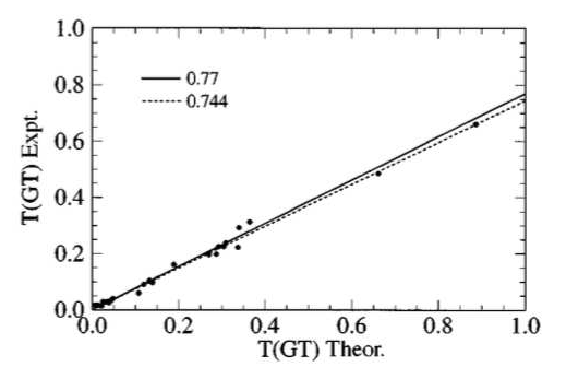
\includegraphics[width=0.5\textwidth]{betaquenching}}
  \subfloat[\tnbb\ Quenching]{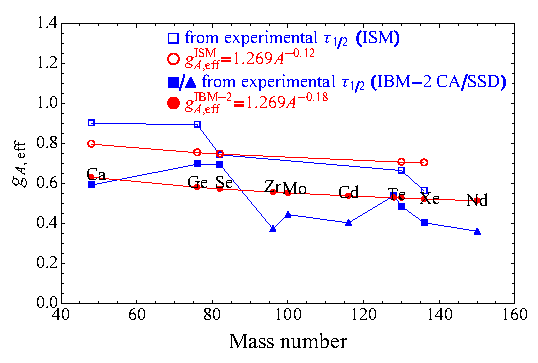
\includegraphics[width=0.5\textwidth]{bbquenching}}
  \caption[$g_A$ Quenching in single- and double-beta decay]{\label{fig:quenching}
    Measurements of single- and double-beta decay Gamow-Teller matrix elements consistently observe smaller values than predicted by theory. This is solved by using an effective $g_A$ that is smaller than the value measured for a free neutron. Taken from \cite{Engel2017}.
  }
\end{figure}

\subsection{Neutrinoless Double-Beta Decay}
\znbb\ is a hypothetical process in which two neutrons become two protons and two electrons, with no accompanying neutrinos.
Because of the lack of neutrinos, all kinetic energy will be carried by electromagnetically interacting particles; if all of the energy is captured in a detector, it will result in a single sharp energy peak at the end-point of the \tnbb\ spectrum (see Figure~\ref{fig:bbspectrum}).
This decay violates lepton number by $\Delta L=2$, requiring BSM physics.
If the neutrino is a Majorana particle, it will induce \znbb\ via the neutrino exchange diagram shown in Figure~\ref{fig:bbdiagram}.
\znbb\ was first suggested as a test of the Majorana nature of neutrinos by Furry in 1939\cite{Furry1939}.
Searches have been performed in ten different isotopes, with no positive results yet.
The most sensitive experiments have half-life limits in the range of $10^{25}-10^{26}$~yrs, in \iso{136}{Xe}\cite{kamlandzen}, \iso{76}{Ge}\cite{gerda2018} and \iso{130}{Te}\cite{Cuore2018}.
\begin{figure}[t]
  \centering
  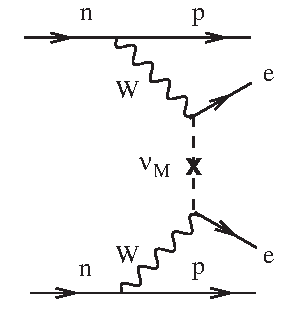
\includegraphics[width=0.3\textwidth]{znbbDiagramLNE}
  \caption[\znbb\ Decay Diagram]{\label{fig:bbdiagram}
    A Feynman diagram for \znbb\ involving the exchange of a light neutrino.
  }
\end{figure}

If \znbb\ is observed, it will unambiguously mean that the neutrino is a Majorana particle.
This is true thanks to the Schechter-Valle theorem (AKA the Black Box theorem), which demonstrates that the \znbb\ diagram itself induces a Majorana mass term as in Figure~\ref{fig:blackbox}\cite{Schechter1982}.
It should be noted that this diagram is a four loop diagram, meaning that the mass induced would be extremely small.
As a result, the discovery of \znbb\ does not necessarily explain fully the origin of neutrino mass.
\begin{figure}[t]
  \centering
  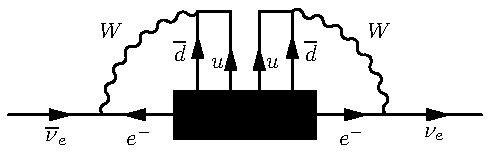
\includegraphics[width=0.8\textwidth]{blackboxdiagram}
  \caption[\znbb\ Decay Diagram]{\label{fig:blackbox}
    The ``black box'' diagram inducing Majorana neutrino mass from \znbb
  }
\end{figure}

\subsection{Calculating Half-life for \znbb\ with Light Neutrino Exchange}
Assuming that light neutrino exchange (LNE), as shown in Figure~\ref{fig:bbdiagram}, is the dominant mechanism causing \znbb, the half-life for \znbb\ can be expressed as:
\begin{equation}
  \frac{1}{T^{0\nu}_{1/2}}=G_{0\nu}(Q,Z)(g_A^{eff,0\nu})^4|M_{0\nu}|^2|m_{\beta\beta}|^2
\end{equation}
This equation is derived and discussed in detail in \cite{Avignone2008, Engel2017}.
The components of this equation, which will mostly be familiar from equation~\ref{eq:2nvvHL}, are as follows:
\begin{itemize}
\item $G_{0\nu}(Q,Z)$ is the phase space factor.
  While the neutrinoless phase space factor differs numerically from the two-neutrino factor, it can be accurately calculated using the same techniques.
\item $|M_{0\nu}|$ is the NME.
  This NME accounts for LNE with a long range, fermion propagator.
  This NME differs significantly from the \tnbb\ NME:
  \begin{equation}
    M_{0\nu}=M^{0\nu}_{GT} - \frac{g_V^2}{g_A^2}M^{0\nu}_F+M^{0\nu}_T
  \end{equation}
  where $M^{0\nu}_T$ is a the Tensor term of the NME.
  Recent work by Cirigliano, \textit{et. al.} suggests that an additional contact term to the NME is also required and may have a value near to leading order\cite{Cirigliano2018_1}.
  The neutrino exchange operator increases the contribution of terms forbidden in the \tnbb\ NMEs, including the Fermi and Tensor terms and intermediate nuclear states beyond the $1^+$ states.
  As a result, the \znbb\ matrix element is very challenging to calculate; as Figure~\ref{fig:horribleplot} shows, different choices of model result in a factor of ${\sim}3$ difference in LNE NMEs.
  Section~\ref{sec:NMEmethods} will describe the differences between these models.
\item $m_{\beta\beta}$ is the effective neutrino mass, expressed as:
  \begin{equation} \label{eq:mbb}
    \begin{aligned}
      m_{\beta\beta}&=\sum_i m_iU_{ei}^2
      &=m_1|U_{e1}|^2+m_2|U_{e2}|^2e^{i(\alpha_2-\alpha_1)}+m_2|U_{e2}|^2e^{-i(\alpha_1+2\delta)}
    \end{aligned}
  \end{equation}
  \begin{figure}[p]
    \centering
    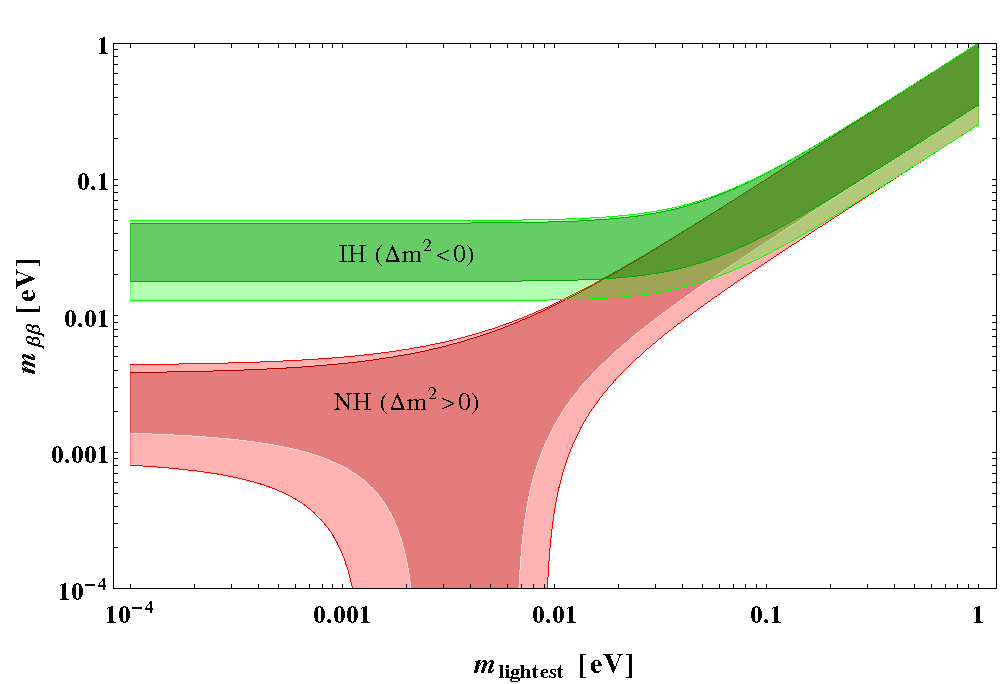
\includegraphics[width=0.95\textwidth]{lobsterplot}
    \caption[Allowed values of $m_{\beta\beta}$]{\label{fig:lobsterplot}
      The allowed values of $m_{\beta\beta}$ based on equation~\ref{eq:mbb} and current experimental constraints from oscillation experiments. $m_{lightest}$ is the mass of the lightest neutrino and can be determined by direct mass measurements or cosmological measurements. The allowed regions can be divided based on the mass ordering into the normal hierarchy (NH) band, the inverted hierarchy (IH) band. The light shaded regions at the boundaries of each band represent the propagation 3-$\sigma$ uncertainties of oscillation parameters\cite{lobsterplot}.
    }
  \end{figure}
  where $m_i$ are the neutrino masses, $U_{ei}$ are the PMNS matrix elements, $\alpha_{1/2}$ and $\delta$ are the CP phases.
  Strictly speaking, this term is included in the NME; however, since the neutrino mass is much smaller than the nuclear scale (${\sim}100$~MeV), it can be separated from the NME.
  This term will be common between all \znbb\ isotopes, and it contains interesting information about both the neutrino mass and leptonic CP violation.
  As a result, $m_{\beta\beta}$ is the target parameter for searches for \znbb, and is how the sensitivity and limits of experiments are compared.
  Figure~\ref{fig:lobsterplot} shows the allowed values of $m_{\beta\beta}$ based on the mass of the lightest neutrino using constraints from oscillation experiments.
  In order to compute a value or limit for $m_{\beta\beta}$ based on a half-life measurement, it is critical to have accurate knowledge of the NME; for this reason, reducing uncertainties and understanding the differences between different NME models is a top priority.
  The current best limit of $m_{\beta\beta}<61-165$~meV has been set by the KamLAND-Zen experiment\cite{kamlandzen}; the factor of three range reflects the uncertainty in the NME. 
\item $g^{eff}_A$ is the quenched $g_A$ coupling.
  While the quenching factor for \tnbb\ has been verified to be similar, its effect on \znbb\ is currently unknown.
  There are good reasons to believe it could be either larger or smaller than the traditional quenching factor, and this adds another factor of ${\sim}3$ uncertainty to the NMEs for all isotopes beyond what is shown in Figure~\ref{fig:horribleplot}\cite{Engel2017}.
  The solution to single-beta $g_A$ quenching suggests an optimistic scenario for \znbb\ and should reduce this uncertainty in the future.
\end{itemize}

\subsection{Calculating Half-life for \znbb\ with Other Physics Mechanisms}
\begin{figure}[t]
  \centering
  \subfloat[\znbb\ Diagrams from LRSM]{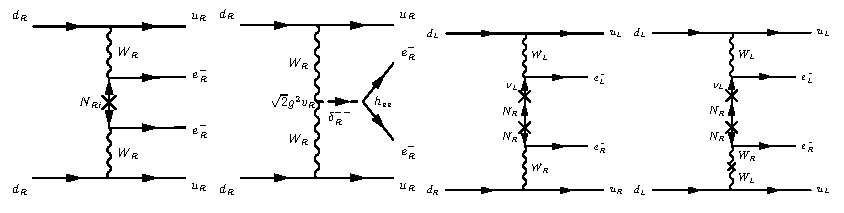
\includegraphics[height=3cm]{znbbDiagramLRSM}}\\
  \subfloat[\znbb\ Diagrams from RPV-SUSY]{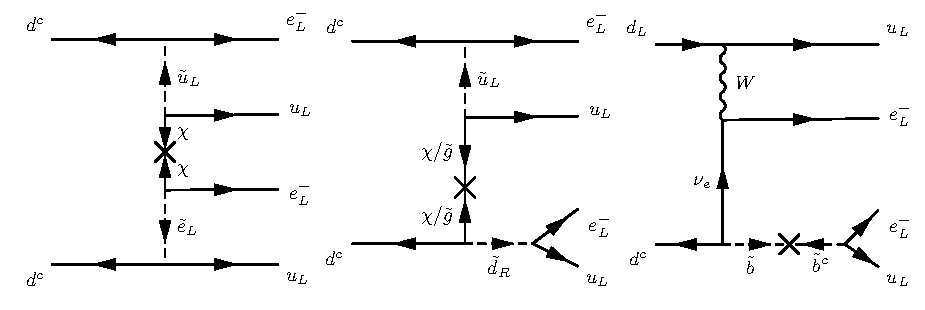
\includegraphics[height=3cm]{znbbDiagramRSUSY}}
  \caption[\znbb\ Diagrams from Heavy BSM Mechanisms]{\label{fig:znbbheavy}
    A sampling of Feynman diagrams for \znbb, assuming exchange of heavy BSM particles. Taken from \cite{Rodejohann2015}.
  }
\end{figure}
The previous section assumed that LNE is the dominant mode for \znbb; however, with many models for generating Majorana neutrino mass, exchanges of other, heavier particles may be the primary decay mode.
In such cases, \znbb\ is not primarily generated by the aforementioned dimension-5 effective Standard Model Lagrangian term, but instead through dimension 6, 7 and 9 terms\cite{Cirigliano2018_2}.
Figure~\ref{fig:znbbheavy} shows a sampling of different BSM particle exchanges that could potentially cause \znbb.
A generic equation for the half-life is:
\begin{equation}
  \frac{1}{T^{0\nu}_{1/2}}=\sum_iG^i_{0\nu}(Q,Z)(g_A^{eff,0\nu})^4|M^i_{0\nu}|^2\eta_i^2
\end{equation}
where $i$ indexes over each mode of \znbb, $G^i_{0\nu}(Q,Z)$ and $M^i_{0\nu}$ are the independant phase space factors and NMEs, and $\eta_i$ includes the new physics parameters.
Because the particles exchanged tend to be heavier than the nuclear scale, the interactions will be short-range or point-like inside the nucleus.
Most heavy-particle exchange interactions will be dominated in an effective theory by the three diagrams in Figure~\ref{fig:znbbeffpion}.
The variety of mechanisms that could lead to \znbb\ means that additional measurements will be required in order to understand the NMEs involved and to measure the physics parameters of interest.
Furthermore, this removes many of the constraints on the half-life that exist with LNE; even so, any of these mechanisms will involve a LNE component as a result of the Schechter-Valle theorem.
This means that, absent fine-tuned destructive interference, these new mechanisms would result in half-lives higher than those predicted for LNE.
\begin{figure}[t]
  \centering
  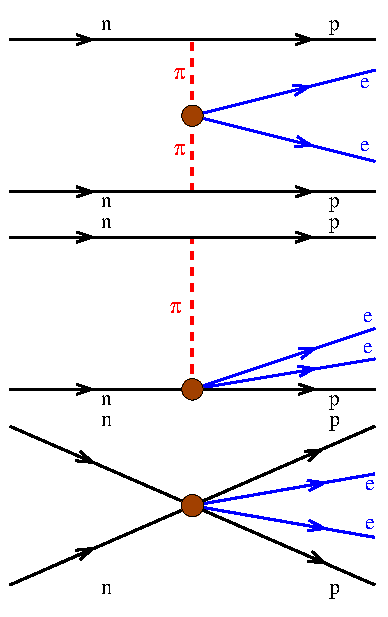
\includegraphics[width=0.4\textwidth]{znbbshortrange}
  \caption[Effective Pion Exchange Operators for \znbb]{\label{fig:znbbeffpion}
    Effective short range operators for generating \znbb. The top two involve pion exchange; the bottom one is the contact operator. These operators are expected to dominate in most BSM \znbb\ mechanisms involving heavy particle exchange. Taken from \cite{Engel2017}.
  }
\end{figure}

\subsection{Nuclear Matrix Elements} \label{sec:NMEmethods}
As previously mentioned, accurate NMEs are critical for interpreting the results of a \znbb\ search.
There is a high degree of uncertainty in the NMEs due to several factors.
First, the mechanism for \znbb\ is unknown; most NMEs are calculated assuming LNE, which will be the focus here.
Second, different models used for calculating NMEs produce results that differ by a factor of ${\sim}3$.
Finally, without understanding the mechanism behind $g_A$ quenching, there is another factor of ${\sim}3$ uncertainty.
This section will discuss many of the models used to produce NMEs; for more complete discussions, see \cite{Avignone2008, Engel2017}.
These techniques can be used for \tnbb\, LNE \znbb\ or \znbb\ by some other mechanism.
Figure~\ref{fig:horribleplot} shows the LNE \znbb\ NMEs calculated by several different theory groups.
\begin{figure}[p]
  \centering
  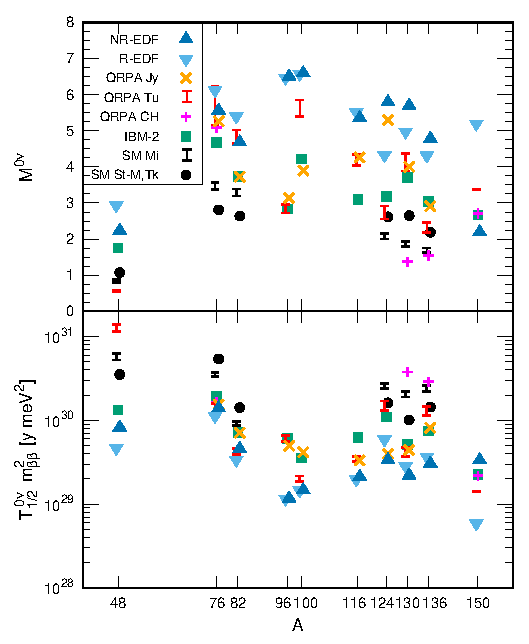
\includegraphics[width=0.8\textwidth]{horribleplot}
  \caption[\znbb\ Nuclear Matrix Element Calculations]{\label{fig:horribleplot}
    Values of LNE NMEs for all \znbb\ isotopes being explored by experiments, using a variety of models. Taken from \cite{Engel2017}.
  }
\end{figure}

The most commonly used NME models are:
\begin{itemize}
\item \textbf{Quasi Random Phase Approximation (QRPA)}: proton-neutron (pn)QRPA is a mean-field based model that uses effective particle-particle and particle-hole operators to model proton and neutron transitions near the Fermi surface.
  QRPA is capable of exploring a large set of valence states, but has trouble accounting fully for nucleon-nucleon correlations.
  Many variants of QRPA exist, incuding renormalized (R)QRPA and multiple commutator model (MCM)-QRPA.
\item \textbf{Shell Model (SM)}: The nuclear shell model attempts to compute Slater determinates using a limited configuration space including nucleon states near the Fermi surface.
  SM is capable of including complex nucleon-nucleon correlations, but the computational complexity grows rapidly with the number of states considered, meaning only a small number of valence states can be included.
\item \textbf{Energy Density Functional (EDF)}: EDF theory attempts to minimize an energy functional with respect to local densities such as the number density $\rho$, spin density $s$, current density $j$, etc.
  The Hamiltonian is minimized, with constraints, over these quantities to obain the energy density functional, which can be used to compute exact nuclear properties.
  EDF theories are not close enough to the exact functionals to accurately compute all quantities in all nuclei and require the explicit inclusion of correlations.
\item \textbf{Interacting Boson Model (IBM)}: IBM utilizes the pairing of nucleons into Bosonic quasi-particles.
  IBM is capable of treating a larger valence space than SM, but loses some degrees of freedom.
\item \textbf{Effective Field Theory (EFT)}: A set of low energy effective many-body operators can be derived and incorporated into many-body calculations using any of the previously mentioned methods.
  Chiral ($\chi$)EFT involves the use of up-to-four body operators, which can be calculated using lattice-QCD.
  One further advantage of this approach is that it is capable of computing errors, unlike the other approaches.
  This method cannot yet be used for \znbb\ NMEs, but there are active attempts to develop this capability.
\end{itemize}
Broadly speaking, there is a tradeoff between the number of valence states that can be included in a calculation and the complexity of correlations that can be included; these differences appear to be responsible for the disagreement between different models.
Ideally, improvements in these different models will eventually lead to greater agreement.
These models are currently incapable of predicting the effect of $g_A$ quenching in \znbb.

\section{Double-Beta Decay to Excited States} \label{sec:bbestheory}
Most \bb\ isotopes can decay into multiple excited states of the daughter nucleus.
Because these are even-even nuclei, these decays will go from a $0^+$ ground state of the parent nucleus to either a $0^+$ or $2^+$ excited state of the daughter.
Because of the higher mass of the excited daughter state, the Q-value of an excited state decay is reduced compared to the ground state decay.
In addition, the daughter will promptly deexcite into the ground state, releasing one or more gamma-rays in the process.
These additional $\gamma$s provide a unique detection signature that can help in searching for \bb-decays to excited states.
Figure~\ref{fig:bbeslevelgeneric} shows a generic $\beta\beta$ decay scheme with three excited states.
\begin{figure}[t]
  \centering
  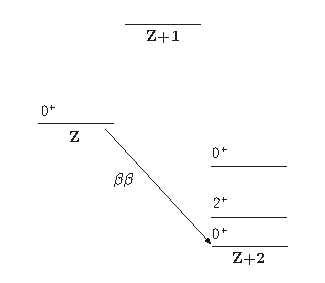
\includegraphics[width=0.5\textwidth]{bbesdecayscheme}
  \caption[Generic $\beta\beta$ to Excited States Level Diagram]{\label{fig:bbeslevelgeneric}
    A generic level diagram for $\beta\beta$-decay, showing multiple excited nuclear daughter states that could result from the decay. This diagram has two excited states (one $0^+$ and one $2^+$).
  }
\end{figure}

Compared to decays to ground states, the rate of excited state decays is suppressed.
To first order, the phase space factor scales with the Q-value $E$ as $E^{11}$ for \tnbb\ and $E^5$ for \znbb; this can suppress the excited state decay rate by many orders of magnitude relative to the ground state decay rates.
Furthermore, for decays to $2^+$ excited states, the change in angular momentum further suppresses the decay rate.

So far, \tnbb\ to first excited $0^+$ states have been observed in \iso{100}{Mo} and \iso{150}{Nd}, but not in any other isotope.
The NME calculations vary significantly depending on what model is used for their calculation.
This means that measurement of \bb -decay to excited states can act as a test for these different models.
So far, observed half-lives have differed significantly from predictions, offering an opportunity to understand sources of error in these calculations.
Because of differences between the \tnbb\ and \znbb\ decay modes previously discussed, such a comparison cannot act as a silver bullet for understanding \znbb\ NMEs.
For a detailed discussion of current experiments and calculations, see \cite{barabash2017}.
Decay to excited states half-lives are also sensitive to additional BSM physics.

\subsection{\tnbb\ NMEs in \Ge{76}} \label{sec:tnbbesnmes}
Table~\ref{tab:Ge76HalfLives} contains a list of theoretical predictions of the half-life of each \tnbb\ excited state decay mode for \Ge{76}.
The models presented use the same techniques and acronyms defined in Section~\ref{sec:NMEmethods}.
For some references included in Table~\ref{tab:Ge76HalfLives}, half-lives were not provided (the IBM\cite{barea2013, barea2015} and EFT\cite{menendez2018}); in these cases, the half-life provided was calculated using:
\begin{equation} \label{eq:hlcalc}
  T^{2\nu~E.S.}_{1/2} = T^{2\nu~G.S.}_{1/2}\cdot\frac{G_{2\nu}^{G.S.}|M_{2\nu}^{G.S.}|^2}{G_{2\nu}^{E.S.}|M_{2\nu}^{E.S.}|^2}
\end{equation}
where $T_{1/2}^{2\nu~g.s.}=1.926\pm0.094\cdot10^{21}$~y is the ground state decay half-life measured by \Gerda\ Phase~I.
$\mathrm{G}_{2\nu}$ are the phase space factors from Mirea, \textit{et al.}\cite{mirea2015}, and $|M_{2\nu}|$ are the matrix elements reported by the given source.
The EFT calculations\cite{menendez2018} also provided error estimates, which tend to be $40-80\%$ for excited state decays and are not shown here.
The half-life predictions for each decay mode of \Ge{76} span many orders of magnitude; this uncertainty is found in all \bb-isotopes\cite{barabash2017}.
This wide range using different techniques is related to a variety of factors, including the nuclear spectroscopy of the the intermediate and final nuclear states, and the physics underlying $g_A$ quenching.
A half-life measurement may prove helpful in understanding some errors of the NME models; optimistically, it may enable improvements in the \znbb\ NME predictions as well.
\begin{table}[p]
  \caption[Current half-live limits and predictions for all \tnbb-decay modes of \Ge{76}]{\label{tab:Ge76HalfLives}
    Table of best half-life predictions and experimental limits for each \Ge{76} \tnbb\ decay mode.}
  \begin{tabular}{|c|r|c c c|}
  \hline
  \tnbb\ Decay Mode & $T^{2\nu\beta\beta}_{1/2}$~(yr) & Experiment/Model & ref. & year \\
  \hline\hline
  \multirow{9}{*}{\makecell{\decaySP{2}{0}{1} \\ \Qbb$=916.8$~keV \\ $559.1 + 563.2$~keV~$\gamma$}}
  & $>3.7\e{23}$ & \Gerda & \cite{gerdaESresult} & 2019 \\
  \cline{2-5}
  & $4.0\e{22}$       & QRPA & \cite{Civitarese1994} & 1994 \\
  & $4.5\e{22}$       & QRPA & \cite{Stoica1996} & 1996 \\
  & $7.5\e{21}$       & MCM-QRPA & \cite{Suhonen1996} & 1996 \\
  & $(1.0-3.1)\e{23}$ & RQRPA & \cite{Suhonen1997} & 1997 \\
  & $(1.2-5.8)\e{23}$ & RQRPA & \cite{gerdaESresult} & 2014 \\
  & $7.1\e{24}$ & IBM-2 & \cite{barea2015} & 2014 \\
  & $(2.3-6.7)\e{24}$ & SM & \cite{gerdaESresult} & 2014 \\
  & $1.7\e{24}$       & EFT & \cite{menendez2018} & 2018 \\
  \hline\hline
  \multirow{9}{*}{\makecell{\decaySP{2}{2}{1} \\ \Qbb$=1480.0$~keV \\ $559.1$~keV~$\gamma$}}
  & $>1.6\e{23}$ & \Gerda & \cite{gerdaESresult} & 2019 \\
  \cline{2-5}
  & $1.2\e{30}$ & SM & \cite{Haxton1984} & 1984 \\
  & $5.8\e{23}$ &  HFB & \cite{dhiman1994} & 1994 \\
  & $5.0\e{26}$ & QRPA & \cite{Civitarese1994} & 1994 \\
  & $2.4\e{24}$ & QRPA & \cite{Stoica1996} & 1996 \\
  & $7.8\e{25}$ & MCM-QRPA & \cite{Suhonen1996} & 1996 \\
  & $1.0\e{26}$ & RQRPA & \cite{Suhonen1997} & 1997 \\
  & $(2.4-4.3)\e{26}$ & RQRPA & \cite{Simkovic1998} & 1998 \\
  & $5.75\e{28}$ & pnQRPA & \cite{Raduta2007} & 2007 \\
  & $2.0\e{27}$ & RQRPA & \cite{Unlu2014} & 2014 \\
  & $1.0\e{27}$ & EFT & \cite{menendez2018} & 2018 \\
  \hline\hline
  \multirow{4}{*}{\makecell{\decaySP{2}{2}{2} \\ \Qbb$=822.0$~keV \\ $64\%: 657.0+559.1$~keV~$\gamma$ \\ $36\%: 1216.1$~keV~$\gamma$}}
  & $>2.3\e{23}$ & \Gerda & \cite{gerdaESresult} & 2019 \\
  \cline{2-5}
  & $1.0\e{29}$ & QRPA & \cite{Civitarese1994} & 1994 \\
  & $1.3\e{29}$ & MCM-QRPA & \cite{Suhonen1996} & 1996 \\
  & $(0.7-2.2)\e{28}$ & RQRPA & \cite{Suhonen1997} & 1997 \\
  \hline
  
\end{tabular}

\end{table}

\subsection{\znbb\ to Excited States}
\begin{figure}[t]
  \centering
  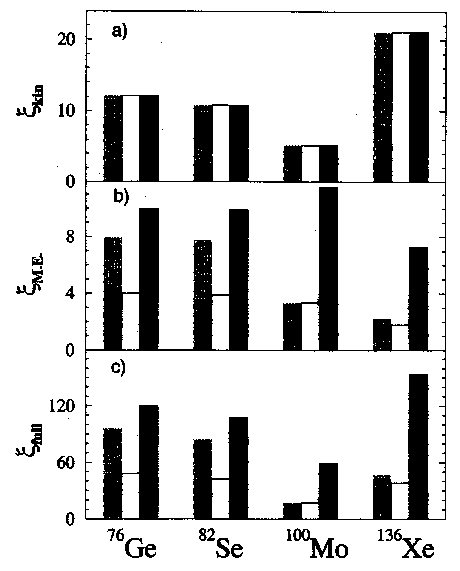
\includegraphics[width=0.7\textwidth]{esmechanismratio}
  \caption[\znbb\ to excited states for different \znbb\ mechanisms]{\label{fig:esmechanism}
    $\xi_{full}$ (bottom) is the ratio of the half-life for the \bb-decay to the first $0^+$ excited state to the ground state. $\xi_{kin}$ (top) and $\xi_{M.E.}$ (middle) are the ratios of the phase space integrals and squared NMEs. This shows a comparison of the rates of \znbb\ to the daughter ground states and first $0^+$ excited states for four different isotopes, using three different mechanisms for producing \znbb. The mechanisms shown are light neutrino exchange (left, textured black), LRSM heavy neutrino exchange (middle, white) and R-parity violating SUSY (right, solid black). Taken from \cite{Simkovic2002}.
  }
\end{figure}
If the neutrino is Majorana, then \znbb\ to excited states can occur.
The NMEs for \znbb\ to excited states vary significantly based on the underlying physics.
It has been further shown that the ratio of the half-lives for \znbb\ to the first $0^+$ excited state and to the ground state varies based on the physics mechanism, as shown in Figure~\ref{fig:esmechanism}\cite{Simkovic2002, Suhonen2016}.
This means that a measurement of both the excited- and ground-state decays could shed light on what BSM physics is causing \znbb.

\subsection{Bosonic Component of Neutrinos} \label{sec:bosonicnus}
If we violate fundamental physical assumptions, including the Pauli exclusion principle and CPT theorems, the neutrino wavefunction could have a bosonic component\cite{Dolgov2005}.
Because of their neutrality and small mass, neutrinos are a strong probe of such physics.
In \tnbb\ to $2^+$ excited states, a bosonic component has been shown to increase the decay rate by approximately an order of magnitude\cite{barabash2007, Tornow2010}.
No search for decays to excited states has yet probed $2^+$ decay half-lives high enough to test this prediction, but in many isotopes, experimental capabilities are improving to the point where this may be feasible.

\section{Summary}
Double-beta decay provides a powerful probe of neutrino physics beyond the Standard Model.
Detection of \znbb\ would indicate that neutrinos are Majorana fermions and provide violation of lepton number.
However, due to the difficulty of computing the nuclear matrix elements, interpretting experimental results becomes difficult.
Detection of \bb -decay to excited states would provide additional data to help improve NME models, and would also potentially open windows to additional BSM physics.
This dissertation will describe the search for \bb -decay to excited states in \Ge{76} using the \MJD.

\onlyinsubfile{
  \bibliographystyle{plain}
  \bibliography{../main}
}

\end{document}
